% The three parts of the Day 1 lab. The steps follow Labs/day01/README.md.
%
% Hardware status: not tested on hardware. A number of this file comes from
% the compiler, from the notebook, or from a source. A value that only a
% board can give is written as "..." and the students measure it.
%
% A menu path stands in one \code command: the character ">" prints
% correctly only in the code font.

% ------------------------------------------------------------------- Part A
\begin{frame}[fragile]{Part A: toolchain (50 min)}
  \small
  \begin{enumerate}
    \item Do steps 1 to 4 of \code{Labs/SETUP.md}: the Arduino IDE, the esp32
          core, the two libraries, the board settings, and the Python
          environment. On Linux, do also step 9 (permission for the USB
          port).
    \item Connect the kit. Click \code{Select Board}, enter \code{xiao}, and
          select \code{XIAO\_ESP32S3} and the port of the board.
    \item Set \code{Tools > PSRAM > Disabled}.
    \item Open \code{sketches/blink/blink.ino}. Click Upload.
    \item Start Jupyter. Run only section 0 (Setup) of the notebook.
  \end{enumerate}
  \begin{lstlisting}[style=shell]
python3 -m venv .venv
.venv/bin/pip install -r Labs/requirements.txt
.venv/bin/jupyter lab Labs/day01/model_budgets.ipynb
\end{lstlisting}
  \textbf{You see:} the versions of Python, \code{numpy}, \code{torch}, and
  \code{torchvision}, and no error.
  \vskip 0.3em
  {\footnotesize\color{coolgray}On Linux, install the CPU version of PyTorch
   first. The README gives the command. On Windows, the programs are in
   \texttt{.venv\textbackslash Scripts\textbackslash}.\par}
\end{frame}

\begin{frame}[fragile]{Part A: Blink gives the first two budgets}
  \textbf{You see:} the built-in LED is on for one second and off for one
  second. The Serial Monitor at 115200 baud prints \code{LED on} and
  \code{LED off}.
  \vskip 0.3em
  Read the last lines of the build output in the Arduino IDE:
  \begin{lstlisting}
Sketch uses 271701 bytes (8%) of program storage space.
    Maximum is 3342336 bytes.
Global variables use 21824 bytes (6%) of dynamic memory,
    leaving 305856 bytes for local variables. Maximum is 327680 bytes.
\end{lstlisting}
  \begingroup\centering
  \begin{tikzpicture}[font=\footnotesize, x=1cm, y=1cm]
    % Bars of 7 cm. Sketch: 8 % of the flash. Global variables: 6 % of the RAM.
    \node[anchor=east] at (-0.1,0.95) {Flash};
    \fill[boxgray] (0,0.75) rectangle (7,1.15);
    \fill[cardinalred!70] (0,0.75) rectangle (0.57,1.15);
    \draw[coolgray] (0,0.75) rectangle (7,1.15);
    \node[anchor=west] at (7.1,0.95) {3 342 336 bytes};
    \node[anchor=west] at (0.65,0.95) {sketch: 271 701 bytes (8 \%)};
    \node[anchor=east] at (-0.1,0.2) {RAM};
    \fill[boxgray] (0,0) rectangle (7,0.4);
    \fill[darkcyan!70] (0,0) rectangle (0.47,0.4);
    \draw[coolgray] (0,0) rectangle (7,0.4);
    \node[anchor=west] at (7.1,0.2) {327 680 bytes};
    \node[anchor=west] at (0.55,0.2) {global variables: 21 824 bytes (6 \%)};
  \end{tikzpicture}\par\endgroup
  \vskip 0.3em
  \begin{itemize}
    \item The first line is the flash budget of a sketch. The second line is
          the RAM budget with no PSRAM.
    \item \textbf{You record:} your two lines. Your numbers can be different.
  \end{itemize}
\end{frame}

% ------------------------------------------------------------------- Part B
\begin{frame}{Part B: five sensor tests (45 min)}
  \footnotesize
  \renewcommand{\arraystretch}{1.2}
  \setlength{\tabcolsep}{4pt}
  \begingroup\centering
  \begin{tabular}{@{}L{0.15\textwidth}L{0.25\textwidth}L{0.16\textwidth}L{0.36\textwidth}@{}}
    \toprule
    \textbf{Test} & \textbf{Sketch} & \textbf{PSRAM} & \textbf{You see} \\
    \midrule
    IMU & \code{imu\_test} & Disabled
      & Six values, ten times each second, in the Serial Monitor \\
    Display & \code{oled\_test} & Disabled
      & \code{Hello} and \code{World!} in a frame on the display \\
    Microphone & \code{mic\_test} & Disabled
      & A line in the Serial Plotter that follows your voice \\
    Camera & \code{camera\_test} & OPI PSRAM
      & One line for each frame, each second \\
    Wi-Fi & \code{WiFiScan} (example) & Disabled
      & The list of the networks with their signal strength \\
    \bottomrule
  \end{tabular}\par\endgroup
  \vskip 0.5em
  \small
  \begin{itemize}
    \item The first four sketches are in \code{Labs/day01/sketches/}.
    \item The serial speed is 115200 baud.
  \end{itemize}
  \keypoint{These five sensors give the data of the later labs. A sensor that
    fails today stops a later lab.}
\end{frame}

\begin{frame}{Part B: IMU and display}
  \begin{columns}[T]
    \begin{column}{0.48\textwidth}
      \centering
      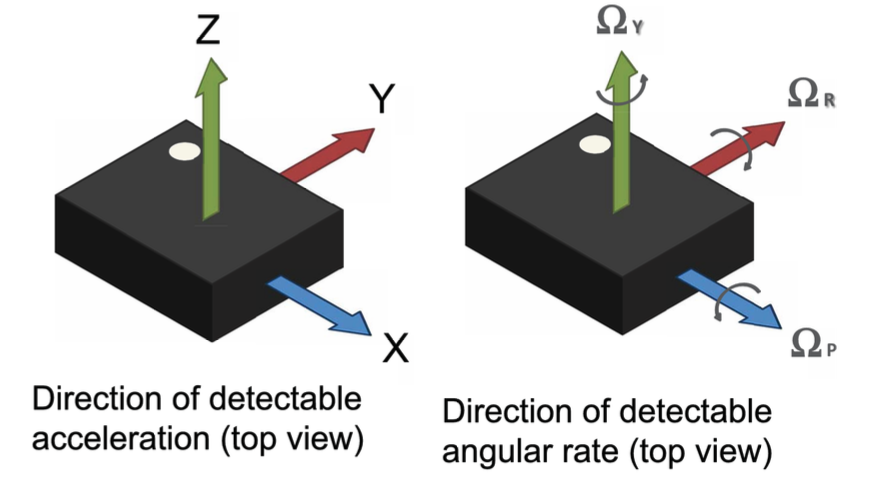
\includegraphics[width=\linewidth]{images/day01/imu-directions.png}
      \vskip 0.6em
      \raggedright\small
      \textbf{Test 2: display}
      \begin{itemize}
        \item Upload \code{oled\_test}.
        \item \textbf{You see:} the text \code{Hello} and \code{World!} in
              a frame on the display of the expansion board.
      \end{itemize}
    \end{column}
    \begin{column}{0.49\textwidth}
      \small
      \textbf{Test 1: IMU}
      \begin{itemize}
        \item Upload \code{imu\_test}. Open the Serial Monitor.
        \item \textbf{You see:} \code{IMU initialized successfully}, then
              six values: the acceleration on three axes and the angular
              rate around three axes.
        \item Put the kit flat on the table: Z is near 1.0 g. X and Y are
              near 0.
        \item Turn the kit on its side: a different axis shows 1.0~g or
              $-$1.0~g.
        \item \textbf{You record:} the Z value with the kit flat.
      \end{itemize}
    \end{column}
  \end{columns}
  \source{Figure and expected values: XIAOML Kit setup chapter of
    \emph{Machine Learning Systems}.}
\end{frame}

\begin{frame}{Part B: microphone and camera}
  \small
  \textbf{Test 3: microphone}
  \begin{itemize}
    \item Upload \code{mic\_test}. Close the Serial Monitor. Open
          \code{Tools > Serial Plotter}.
    \item \textbf{You see:} small values in silence. Speak or clap: the line
          shows large positive and negative values.
  \end{itemize}
  \textbf{Test 4: camera}
  \begin{exerciseblock}
    \textbf{Predict before the test.} One frame has 320 $\times$ 240 pixels
    with one byte for each pixel. How many bytes has one frame? Does one
    frame fit in the RAM of a microcontroller with 256 KB?
  \end{exerciseblock}
  \begin{itemize}
    \item Set \code{Tools > PSRAM > OPI PSRAM}. Upload \code{camera\_test}.
    \item \textbf{You see:} \code{Camera initialized}, then one line each
          second with these five values:
          \code{width,height,bytes,capture\_ms,mean\_brightness}
    \item Cover the lens: the last value decreases. A lamp: it increases.
    \item \textbf{You record:} the bytes of one frame and the capture time.
  \end{itemize}
\end{frame}

\begin{frame}[fragile]{Part B: Wi-Fi}
  \begin{columns}[T]
    \begin{column}{0.27\textwidth}
      \centering
      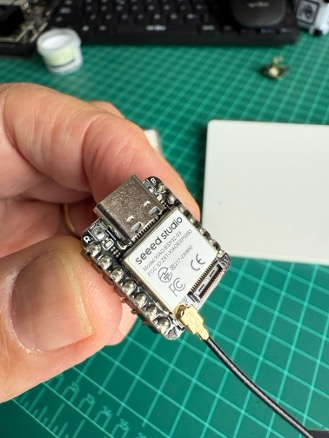
\includegraphics[width=\linewidth]{images/day01/antenna.jpg}
    \end{column}
    \begin{column}{0.69\textwidth}
      \small
      \textbf{Test 5: Wi-Fi}
      \begin{itemize}
        \item Connect the antenna to the small connector on the XIAO. Put
              one side of the antenna connector in first. Then press the
              other side down.
        \item Open \code{File > Examples > WiFi > WiFiScan}. Upload it. The
              example needs no password.
        \item \textbf{You see:} a list of this form.
      \end{itemize}
      \begin{lstlisting}
Scan start
Scan done
2 networks found
Nr | SSID          | RSSI | CH | Encryption
 1 | ...           |  ... | .. | ...
\end{lstlisting}
      \begin{itemize}
        \item \textbf{You record:} the number of networks and the RSSI of
              the strongest network.
      \end{itemize}
    \end{column}
  \end{columns}
  \vskip 0.4em
  \small
  RSSI is the signal strength in dBm. A value nearer to 0 is a stronger
  signal.
  \source{Photograph: XIAOML Kit setup chapter of \emph{Machine Learning
    Systems}.}
\end{frame}

% ------------------------------------------------------------------- Part C
\begin{frame}[fragile]{Part C: the memory of the board (10 min)}
  \small
  \begin{enumerate}
    \item Set \code{Tools > PSRAM > Disabled}. Upload
          \code{sketches/memory\_report}. Record the three values of the
          heap.
    \item Set \code{Tools > PSRAM > OPI PSRAM}. Upload again. Record the
          same three values and the two values of the PSRAM.
  \end{enumerate}
  \begin{lstlisting}
--- Internal RAM (heap) ---
Heap size                                 ... bytes    ... KB    <- record
Free heap                                 ... bytes    ... KB    <- record
Lowest free heap since start              ... bytes    ... KB
Largest block that malloc can give        ... bytes    ... KB    <- record
--- External RAM (PSRAM) ---
PSRAM size                                ... bytes    ... KB    <- record
Free PSRAM                                ... bytes    ... KB    <- record
\end{lstlisting}
  \begin{itemize}
    \item ``Largest block that malloc can give'' is your RAM budget with no
          PSRAM. A model needs one block for all its tensors.
    \item ``Free PSRAM'' is your RAM budget with PSRAM.
  \end{itemize}
  \keypoint{You measure the budget. The 8 MB of the data sheet is not the
    free memory.}
  \source{Form of the output of \texttt{memory\_report}.}
\end{frame}

\begin{frame}[fragile]{Part C: the notebook (35 min)}
  \small
  Open \code{model\_budgets.ipynb}. Each task has the mark
  \code{TODO (student)}.
  \vskip 0.3em
  \footnotesize
  \renewcommand{\arraystretch}{1.2}
  \setlength{\tabcolsep}{4pt}
  \begingroup\centering
  \begin{tabular}{@{}lL{0.62\textwidth}L{0.22\textwidth}@{}}
    \toprule
    \textbf{Task} & \textbf{Work} & \textbf{Notebook} \\
    \midrule
    1 & Write the function \code{conv\_cost}: the cost of one convolution
        layer & Section 1 \\
    2 & Write your predictions for three models & Section 3 \\
    3 & Put your two measured RAM budgets of the XIAO in the device table
      & Section 5 \\
    4 & Write the function \code{fits}: does a model fit a device?
      & Section 5 \\
    5 & Write the Decision Log & Section 6 \\
    \bottomrule
  \end{tabular}\par\endgroup
  \vskip 0.4em
  \small
  The check cell of task 1 compares your function with PyTorch:
  \begin{lstlisting}
standard, stride 2: correct
    expected (48, 48, 448, 995328)
    yours    (48, 48, 448, 995328)
...
Task 1: complete
\end{lstlisting}
  The four numbers are: output height, output width, parameters, MACs.
\end{frame}

\begin{frame}{Part C: predict, then profile}
  \small
  \code{profile\_model} gives the three budgets of a model. For the example
  network of the lecture: 24 234 parameters, 6 304 384 MACs, and a peak of
  64 512 values.
  \vskip 0.3em
  \footnotesize
  \renewcommand{\arraystretch}{1.15}
  \setlength{\tabcolsep}{4pt}
  \begin{tabular}{@{}llL{0.50\textwidth}@{}}
    \toprule
    \textbf{Model} & \textbf{Input} & \textbf{Design} \\
    \midrule
    MobileNetV2 & 224 $\times$ 224 $\times$ 3
      & Inverted residual blocks, for phones \\
    ResNet-18 & 224 $\times$ 224 $\times$ 3
      & Standard convolutions with skip connections \\
    Small depthwise CNN & 96 $\times$ 96 $\times$ 3
      & Depthwise separable blocks, for a microcontroller \\
    \bottomrule
  \end{tabular}
  \vskip 0.3em
  \small
  \begin{exerciseblock}
    \textbf{Task 2: predict before you run section 4.}
    \begin{itemize}
      \item Which model has the most parameters?
      \item Which model has the most operations (MACs)?
      \item Which model has the largest peak activation memory?
      \item What is the ratio of the parameters, ResNet-18 to MobileNetV2?
    \end{itemize}
  \end{exerciseblock}
  A wrong prediction costs no points. A missing prediction does.
  \source{Models: \texttt{torchvision} (BSD-3-Clause).}
\end{frame}

\begin{frame}{Part C: does the model fit the device?}
  \begingroup\centering
  \begin{tikzpicture}[font=\footnotesize, >={Stealth[length=5pt]},
      bx/.style={draw=darkcyan, line width=0.8pt, rounded corners=3pt,
                 fill=boxgray, minimum width=4.6cm, minimum height=1.0cm,
                 align=center},
      res/.style={draw=treegreen, line width=0.8pt, rounded corners=3pt,
                  fill=boxgray, minimum width=1.9cm, minimum height=1.0cm,
                  align=center}]
    \node[bx]  (f) at (0,0.65)  {\textbf{Flash:} model size $+$ 300 KB\\
                                 program $\leq$ flash of the device};
    \node[bx]  (r) at (0,-0.65) {\textbf{RAM:} peak activation memory\\
                                 $\leq$ RAM for tensors};
    \node[res] (y) at (4.9,0)   {\textbf{fits}};
    \draw[->] (f.east) -- node[above, sloped] {yes} (y.north west);
    \draw[->] (r.east) -- node[below, sloped] {yes} (y.south west);
    \node[anchor=west, align=left, text=cardinalred] at (6.0,0)
      {One ``no'':\\does not fit.\\Give the reason.};
  \end{tikzpicture}\par\endgroup
  \vskip 0.3em
  \footnotesize
  \renewcommand{\arraystretch}{1.2}
  \setlength{\tabcolsep}{3pt}
  \begingroup\centering
  \begin{tabular}{@{}L{0.31\textwidth}rrL{0.39\textwidth}@{}}
    \toprule
    \textbf{Device} & \textbf{Flash} & \textbf{RAM}
      & \textbf{Source of the RAM value} \\
    \midrule
    Microcontroller, 256 KB & 1.0 MB & 211.1 KB
      & 256 KB less the static RAM of a sensor sketch \\
    XIAO, no PSRAM & 3.2 MB & 298.7 KB
      & Result of the compiler. Task 3: your ``largest block''. \\
    XIAO, with PSRAM & 3.2 MB & 8.0 MB
      & Size of the chip. Task 3: your ``free PSRAM''. \\
    Raspberry Pi 5 & 64 GB & 8 GB
      & microSD card and RAM of the board \\
    \bottomrule
  \end{tabular}\par\endgroup
  \vskip 0.2em
  \small
  \textbf{You record:} six rows (three models in \code{float32} and in
  \code{int8}) for four devices. Each ``does not fit'' has a reason: flash,
  RAM, or flash and RAM.
  \source{Device budgets of the notebook \texttt{model\_budgets.ipynb}.}
\end{frame}
